\documentclass{article}

\usepackage{explorations}

\lesson{Powers of 2, \nicefrac12, and 10}

\begin{document}

\let\oldfn\thefootnote
\renewcommand{\thefootnote}{\fnsymbol{footnote}}
\section*{Powers of 2}

\subsection*{How fast can rumors spread by word of mouth?}
If you tell 2 friends, and they tell 2 friends, and so on, how fast can a rumor spread just by word of mouth?

\begin{enumerate}
\item Watch the following two commercials and compare the two videos in terms of powers of 2.

  \begin{tabular}{lr}
    \url{https://youtu.be/DKUZx1Nk4yY} Faberge shampoo commercial &\qrcode{https://youtu.be/DKUZx1Nk4yY}\\
    & \\
    \url{https://youtu.be/JA7CKvoKEmE} Wayne’s World parody & \qrcode{https://youtu.be/JA7CKvoKEmE}
  \end{tabular}


  \vfill
  
\item Let's first calculate some powers of 2 to warm up.
  \[      \renewcommand{\arraystretch}{2}
    \begin{array}{rcccl}
      2^1 & = &\text{\underline{\hspace{0.5in}}}&&\\
      2^2 & = & 2\cdot 2 & = & \text{\underline{\hspace{0.5in}}}\\
      2^3 & = & 2\cdot 2\cdot 2 &= & \text{\underline{\hspace{0.5in}}}\\
      2^4 & = & \text{\underline{\hspace{0.75in}}} & = & \text{\underline{\hspace{0.5in}}}\\
      2^5 & = & \text{\underline{\hspace{0.75in}}} & = & \text{\underline{\hspace{0.5in}}}
    \end{array}
  \]
\item City College has about 16000 students\footnote{
    \url{http://research.sdccd.edu/docs/Student\%20Profiles/Demographics/20171/Student\%20Profile\%20CR-20171_CD.pdf}}. How many iterations of ``telling''need to occur before the entire student body hears the rumor?

  \vfill

  \clearpage
\item If each cycle took one hour, then in \underline{\hspace{0.5in}} hours, the whole school would know. What if each cycle took 15 minutes? Is this surprising?

  \vfill
  
\item Discuss with a neighbor how social media would affect the spread of rumors. Any
  personal experiences you can share?

  \vfill
  
\end{enumerate}
\section*{Powers of \nicefrac{1}{2}}

We have just seen how quickly powers of 2 can grow. Now we will do a hands-on activity that goes in the opposite direction --- powers of \nicefrac{1}{2}. Your instructor will give your group a square piece of paper with scissors and tape. Try to construct the following image using the materials given. Label each piece with the correct power of 2. For instance, \(\nicefrac12\) is \(\pqty{\nicefrac12}^1\) and \(\nicefrac14\) is \(\pqty{\nicefrac12}^2\)

\begin{center}
  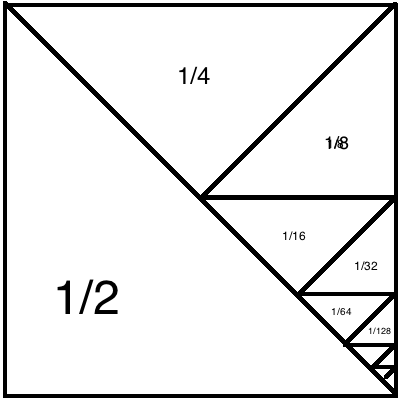
\includegraphics[width=0.25\textwidth]{square.png}
\end{center}
\begin{enumerate}[resume]
\item How many powers of \nicefrac{1}{2} were you able to physically create?

  \vfill
  
\item Where would you encounter powers of \nicefrac{1}{2} in real life?

  \vfill
  
\end{enumerate}

\section*{Powers of 10}

We will now watch two powers of 10 videos: \url{http://www.eamesoffice.com/education/powers-of-ten-2/}\footnote{\hphantom{ab} \qrcode{http://www.eamesoffice.com/education/powers-of-ten-2/}}

\mynewpage

\ \hfill Name: \underline{\hspace{1.5in}}

\section*{Homework Exercises}

\begin{enumerate}
\item Find the following powers of 10 or missing exponent.

  \begin{equation*}
    \renewcommand{\arraystretch}{2}
    \begin{array}{|c|c|}
      \hline 10^1 & 10\\
      \hline 10^2 & 10\cdot 10 = 100\\
      \hline 10^3 & 10\cdot 10\cdot 10 = 1000\\
      \hline 10^4 & \\
      \hline 10^5 & \\
      \hline 10^6 & \\
      \hline 10^{{\text{\ }}^{\fbox{\phantom{1000}}}} & 1,000,000,000\\
      \hline 10^{{\text{\ }}^{\fbox{\phantom{1000}}}} & 10,000,000,000,000\\
      \hline
    \end{array}
  \end{equation*}
\item Do you notice any pattern or relationship between the exponent and the number of zeroes?

  \vfill
  
\item How many seconds are in one minute?

  \vfill
  
\item If you could say two numbers in one second, how many numbers could you say in one minute? (Show the setup of your calculation.)

  \vfill
  
\item How many minutes are in one hour?

  \vfill
  
\item If you could say two numbers in one second, how many numbers could you say in one hour? (Show the setup of your calculation.)

  \vfill

  \clearpage
\item How many hours would you need to count to one billion? (Show the setup of your calculation.)

  \vspace{1in}

\item Why would it take 4 to 5 days to count to one billion? (Show the setup of your calculation.)

  \vspace{1in}
  
\item How long would it take to count to one billion if you said 2 numbers every second? Can you realistically say 2 large numbers in one second?
\end{enumerate}

\renewcommand{\thefootnote}{\oldfn}
\end{document}

%%% Local Variables:
%%% mode: latex
%%% TeX-master: t
%%% End:
